% Options for packages loaded elsewhere
\PassOptionsToPackage{unicode}{hyperref}
\PassOptionsToPackage{hyphens}{url}
\PassOptionsToPackage{dvipsnames,svgnames,x11names}{xcolor}
%
\documentclass[
  letterpaper,
  DIV=11,
  numbers=noendperiod]{scrreprt}

\usepackage{amsmath,amssymb}
\usepackage{iftex}
\ifPDFTeX
  \usepackage[T1]{fontenc}
  \usepackage[utf8]{inputenc}
  \usepackage{textcomp} % provide euro and other symbols
\else % if luatex or xetex
  \usepackage{unicode-math}
  \defaultfontfeatures{Scale=MatchLowercase}
  \defaultfontfeatures[\rmfamily]{Ligatures=TeX,Scale=1}
\fi
\usepackage{lmodern}
\ifPDFTeX\else  
    % xetex/luatex font selection
\fi
% Use upquote if available, for straight quotes in verbatim environments
\IfFileExists{upquote.sty}{\usepackage{upquote}}{}
\IfFileExists{microtype.sty}{% use microtype if available
  \usepackage[]{microtype}
  \UseMicrotypeSet[protrusion]{basicmath} % disable protrusion for tt fonts
}{}
\makeatletter
\@ifundefined{KOMAClassName}{% if non-KOMA class
  \IfFileExists{parskip.sty}{%
    \usepackage{parskip}
  }{% else
    \setlength{\parindent}{0pt}
    \setlength{\parskip}{6pt plus 2pt minus 1pt}}
}{% if KOMA class
  \KOMAoptions{parskip=half}}
\makeatother
\usepackage{xcolor}
\setlength{\emergencystretch}{3em} % prevent overfull lines
\setcounter{secnumdepth}{5}
% Make \paragraph and \subparagraph free-standing
\ifx\paragraph\undefined\else
  \let\oldparagraph\paragraph
  \renewcommand{\paragraph}[1]{\oldparagraph{#1}\mbox{}}
\fi
\ifx\subparagraph\undefined\else
  \let\oldsubparagraph\subparagraph
  \renewcommand{\subparagraph}[1]{\oldsubparagraph{#1}\mbox{}}
\fi

\usepackage{color}
\usepackage{fancyvrb}
\newcommand{\VerbBar}{|}
\newcommand{\VERB}{\Verb[commandchars=\\\{\}]}
\DefineVerbatimEnvironment{Highlighting}{Verbatim}{commandchars=\\\{\}}
% Add ',fontsize=\small' for more characters per line
\usepackage{framed}
\definecolor{shadecolor}{RGB}{241,243,245}
\newenvironment{Shaded}{\begin{snugshade}}{\end{snugshade}}
\newcommand{\AlertTok}[1]{\textcolor[rgb]{0.68,0.00,0.00}{#1}}
\newcommand{\AnnotationTok}[1]{\textcolor[rgb]{0.37,0.37,0.37}{#1}}
\newcommand{\AttributeTok}[1]{\textcolor[rgb]{0.40,0.45,0.13}{#1}}
\newcommand{\BaseNTok}[1]{\textcolor[rgb]{0.68,0.00,0.00}{#1}}
\newcommand{\BuiltInTok}[1]{\textcolor[rgb]{0.00,0.23,0.31}{#1}}
\newcommand{\CharTok}[1]{\textcolor[rgb]{0.13,0.47,0.30}{#1}}
\newcommand{\CommentTok}[1]{\textcolor[rgb]{0.37,0.37,0.37}{#1}}
\newcommand{\CommentVarTok}[1]{\textcolor[rgb]{0.37,0.37,0.37}{\textit{#1}}}
\newcommand{\ConstantTok}[1]{\textcolor[rgb]{0.56,0.35,0.01}{#1}}
\newcommand{\ControlFlowTok}[1]{\textcolor[rgb]{0.00,0.23,0.31}{#1}}
\newcommand{\DataTypeTok}[1]{\textcolor[rgb]{0.68,0.00,0.00}{#1}}
\newcommand{\DecValTok}[1]{\textcolor[rgb]{0.68,0.00,0.00}{#1}}
\newcommand{\DocumentationTok}[1]{\textcolor[rgb]{0.37,0.37,0.37}{\textit{#1}}}
\newcommand{\ErrorTok}[1]{\textcolor[rgb]{0.68,0.00,0.00}{#1}}
\newcommand{\ExtensionTok}[1]{\textcolor[rgb]{0.00,0.23,0.31}{#1}}
\newcommand{\FloatTok}[1]{\textcolor[rgb]{0.68,0.00,0.00}{#1}}
\newcommand{\FunctionTok}[1]{\textcolor[rgb]{0.28,0.35,0.67}{#1}}
\newcommand{\ImportTok}[1]{\textcolor[rgb]{0.00,0.46,0.62}{#1}}
\newcommand{\InformationTok}[1]{\textcolor[rgb]{0.37,0.37,0.37}{#1}}
\newcommand{\KeywordTok}[1]{\textcolor[rgb]{0.00,0.23,0.31}{#1}}
\newcommand{\NormalTok}[1]{\textcolor[rgb]{0.00,0.23,0.31}{#1}}
\newcommand{\OperatorTok}[1]{\textcolor[rgb]{0.37,0.37,0.37}{#1}}
\newcommand{\OtherTok}[1]{\textcolor[rgb]{0.00,0.23,0.31}{#1}}
\newcommand{\PreprocessorTok}[1]{\textcolor[rgb]{0.68,0.00,0.00}{#1}}
\newcommand{\RegionMarkerTok}[1]{\textcolor[rgb]{0.00,0.23,0.31}{#1}}
\newcommand{\SpecialCharTok}[1]{\textcolor[rgb]{0.37,0.37,0.37}{#1}}
\newcommand{\SpecialStringTok}[1]{\textcolor[rgb]{0.13,0.47,0.30}{#1}}
\newcommand{\StringTok}[1]{\textcolor[rgb]{0.13,0.47,0.30}{#1}}
\newcommand{\VariableTok}[1]{\textcolor[rgb]{0.07,0.07,0.07}{#1}}
\newcommand{\VerbatimStringTok}[1]{\textcolor[rgb]{0.13,0.47,0.30}{#1}}
\newcommand{\WarningTok}[1]{\textcolor[rgb]{0.37,0.37,0.37}{\textit{#1}}}

\providecommand{\tightlist}{%
  \setlength{\itemsep}{0pt}\setlength{\parskip}{0pt}}\usepackage{longtable,booktabs,array}
\usepackage{calc} % for calculating minipage widths
% Correct order of tables after \paragraph or \subparagraph
\usepackage{etoolbox}
\makeatletter
\patchcmd\longtable{\par}{\if@noskipsec\mbox{}\fi\par}{}{}
\makeatother
% Allow footnotes in longtable head/foot
\IfFileExists{footnotehyper.sty}{\usepackage{footnotehyper}}{\usepackage{footnote}}
\makesavenoteenv{longtable}
\usepackage{graphicx}
\makeatletter
\def\maxwidth{\ifdim\Gin@nat@width>\linewidth\linewidth\else\Gin@nat@width\fi}
\def\maxheight{\ifdim\Gin@nat@height>\textheight\textheight\else\Gin@nat@height\fi}
\makeatother
% Scale images if necessary, so that they will not overflow the page
% margins by default, and it is still possible to overwrite the defaults
% using explicit options in \includegraphics[width, height, ...]{}
\setkeys{Gin}{width=\maxwidth,height=\maxheight,keepaspectratio}
% Set default figure placement to htbp
\makeatletter
\def\fps@figure{htbp}
\makeatother
\newlength{\cslhangindent}
\setlength{\cslhangindent}{1.5em}
\newlength{\csllabelwidth}
\setlength{\csllabelwidth}{3em}
\newlength{\cslentryspacingunit} % times entry-spacing
\setlength{\cslentryspacingunit}{\parskip}
\newenvironment{CSLReferences}[2] % #1 hanging-ident, #2 entry spacing
 {% don't indent paragraphs
  \setlength{\parindent}{0pt}
  % turn on hanging indent if param 1 is 1
  \ifodd #1
  \let\oldpar\par
  \def\par{\hangindent=\cslhangindent\oldpar}
  \fi
  % set entry spacing
  \setlength{\parskip}{#2\cslentryspacingunit}
 }%
 {}
\usepackage{calc}
\newcommand{\CSLBlock}[1]{#1\hfill\break}
\newcommand{\CSLLeftMargin}[1]{\parbox[t]{\csllabelwidth}{#1}}
\newcommand{\CSLRightInline}[1]{\parbox[t]{\linewidth - \csllabelwidth}{#1}\break}
\newcommand{\CSLIndent}[1]{\hspace{\cslhangindent}#1}

\KOMAoption{captions}{tableheading}
\makeatletter
\makeatother
\makeatletter
\@ifpackageloaded{bookmark}{}{\usepackage{bookmark}}
\makeatother
\makeatletter
\@ifpackageloaded{caption}{}{\usepackage{caption}}
\AtBeginDocument{%
\ifdefined\contentsname
  \renewcommand*\contentsname{Table of contents}
\else
  \newcommand\contentsname{Table of contents}
\fi
\ifdefined\listfigurename
  \renewcommand*\listfigurename{List of Figures}
\else
  \newcommand\listfigurename{List of Figures}
\fi
\ifdefined\listtablename
  \renewcommand*\listtablename{List of Tables}
\else
  \newcommand\listtablename{List of Tables}
\fi
\ifdefined\figurename
  \renewcommand*\figurename{Figure}
\else
  \newcommand\figurename{Figure}
\fi
\ifdefined\tablename
  \renewcommand*\tablename{Table}
\else
  \newcommand\tablename{Table}
\fi
}
\@ifpackageloaded{float}{}{\usepackage{float}}
\floatstyle{ruled}
\@ifundefined{c@chapter}{\newfloat{codelisting}{h}{lop}}{\newfloat{codelisting}{h}{lop}[chapter]}
\floatname{codelisting}{Listing}
\newcommand*\listoflistings{\listof{codelisting}{List of Listings}}
\usepackage{amsthm}
\theoremstyle{definition}
\newtheorem{definition}{Definition}[chapter]
\theoremstyle{definition}
\newtheorem{example}{Example}[chapter]
\theoremstyle{plain}
\newtheorem{theorem}{Theorem}[chapter]
\theoremstyle{remark}
\AtBeginDocument{\renewcommand*{\proofname}{Proof}}
\newtheorem*{remark}{Remark}
\newtheorem*{solution}{Solution}
\makeatother
\makeatletter
\@ifpackageloaded{caption}{}{\usepackage{caption}}
\@ifpackageloaded{subcaption}{}{\usepackage{subcaption}}
\makeatother
\makeatletter
\@ifpackageloaded{tcolorbox}{}{\usepackage[skins,breakable]{tcolorbox}}
\makeatother
\makeatletter
\@ifundefined{shadecolor}{\definecolor{shadecolor}{rgb}{.97, .97, .97}}
\makeatother
\makeatletter
\makeatother
\makeatletter
\makeatother
\ifLuaTeX
  \usepackage{selnolig}  % disable illegal ligatures
\fi
\IfFileExists{bookmark.sty}{\usepackage{bookmark}}{\usepackage{hyperref}}
\IfFileExists{xurl.sty}{\usepackage{xurl}}{} % add URL line breaks if available
\urlstyle{same} % disable monospaced font for URLs
\hypersetup{
  pdftitle={Series temporais},
  pdfauthor={James D Santos},
  colorlinks=true,
  linkcolor={blue},
  filecolor={Maroon},
  citecolor={Blue},
  urlcolor={Blue},
  pdfcreator={LaTeX via pandoc}}

\title{Series temporais}
\author{James D Santos}
\date{2023-02-12}

\begin{document}
\maketitle
\ifdefined\Shaded\renewenvironment{Shaded}{\begin{tcolorbox}[frame hidden, boxrule=0pt, borderline west={3pt}{0pt}{shadecolor}, sharp corners, enhanced, interior hidden, breakable]}{\end{tcolorbox}}\fi

\renewcommand*\contentsname{Table of contents}
{
\hypersetup{linkcolor=}
\setcounter{tocdepth}{2}
\tableofcontents
}
\bookmarksetup{startatroot}

\hypertarget{preface}{%
\chapter*{Preface}\label{preface}}
\addcontentsline{toc}{chapter}{Preface}

\markboth{Preface}{Preface}

This is a Quarto book.

To learn more about Quarto books visit
\url{https://quarto.org/docs/books}.

\begin{Shaded}
\begin{Highlighting}[]
\DecValTok{1} \SpecialCharTok{+} \DecValTok{1}
\end{Highlighting}
\end{Shaded}

\begin{verbatim}
[1] 2
\end{verbatim}

\bookmarksetup{startatroot}

\hypertarget{introduuxe7uxe3o}{%
\chapter{Introdução}\label{introduuxe7uxe3o}}

\hypertarget{notauxe7uxf5es}{%
\section{Notações}\label{notauxe7uxf5es}}

Serão utilizadas letras minúsculas para designar tanto variáveis
aleatórias quanto seus respectivos valores observados, entando a
diferença clara no contexto. Exemplo: em \[x_t\sim\hbox{Normal}(0,1),\]
\(x_t\) representa uma variável aleatória, enquanto que em \(x_t=0\) é
um valor observado.

Vetores serão denotados por negritos e sempre serão vetores-coluna.
Exemplo
\[\boldsymbol{x}=\left(\begin{array}{c}x_1 \\ x_2 \\ \vdots \\ x_q\end{array}\right).\]
O vetor \(\boldsymbol{x}'\) é o transposto de \(\boldsymbol{x}\).

Para \(\mathcal{T}=\{1,2\ldots,\}\),

\begin{itemize}
\tightlist
\item
  Se \(A\subset\mathcal{T}\). Então \(x_A=\{x_{t},t\in A\}\).
\item
  \(x_{a:b}=x_a,x_{a+1},\ldots,x_{b-1},x_{b}.\)
\item
  Um vetor de dimensão \(q\) observado no tempo \(t\) é escrito como
  \[\boldsymbol{x}_t =\left(\begin{array}{c}x_{1} \\ \vdots \\ x_{q}\end{array}\right)_{t}.\]
\end{itemize}

\hypertarget{o-que-uxe9-uma-anuxe1lise-de-suxe9ries-temporais}{%
\section{O que é uma análise de séries
temporais?}\label{o-que-uxe9-uma-anuxe1lise-de-suxe9ries-temporais}}

Considera-se que uma série temporal é uma coleção de observações
realizadas ao longo do tempo. Será utilizada a notação \(x_t\) para
designar o valor registrado no tempo \(t\) e
\(\mathcal{D}_t=}=\{x_1,\ldots,x_t\}\) representará a série observada
até o tempo \(t\).

Existem três objetivos principais no estudo de séries temporais

\begin{itemize}
\item
  \emph{Previsão:} Dado \(\mathcal{D}_t\) a previsão trata do problema
  de realizar inferências sobre \(x_{t+h}\), com \(h>0\).
\item
  \emph{Suavização (ou alisamento):} Dado \(\mathcal{D}_t\) a suavização
  trata do problema de realizar inferências baseadas \(x_{t-h}\), com
  \(h>0\)
\item
  \emph{Monitoramento:} detectar em tempo real as mudanças ou
  discrepâncias no comportamento do processo.
\end{itemize}

Note que tais objetivos só fazem sentido se há alguma estrutura de
dependência entre as variáveis que compõe a série temporal. Para
ilustrar, considere a figura abaixo representa o gráfico a série
temporal com o número anual de embarques e desembarques de passageiros
em vôos domésticos no aeroporto Eduardo Gomes.

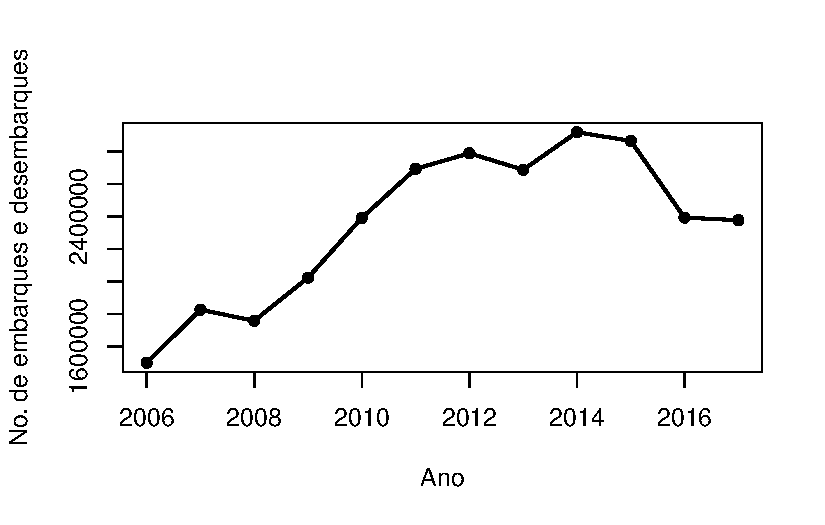
\includegraphics{intro_files/figure-pdf/unnamed-chunk-1-1.pdf}

Ainda considerando a série acima, seja \(x_t\) o número de embarques e
desembarques registrado no ano \(t\). A figura abaixo mostra o diagrama
de disperão entre \(x_t\) e \(x_{t-1}\), de onde é possível observar a
correlação positiva, estimada em 0,86.

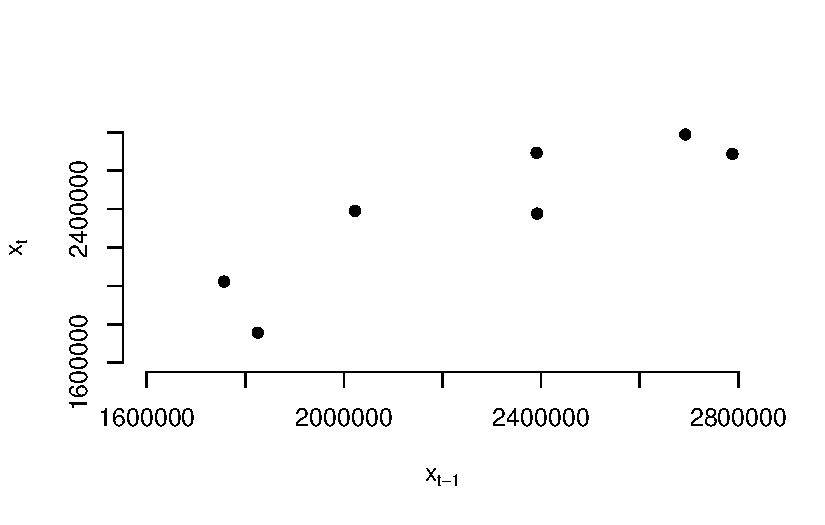
\includegraphics{intro_files/figure-pdf/unnamed-chunk-2-1.pdf}

De posse desses resultados, pode-se imaginar um primeiro modelo, no qual
a relação entre o presente e o passado imediato é ditado por uma
regressão linear simples, gerando a equação

\[\hat{x}_t = 7,589\times 10^5 +0,7109 x_{t-1}.\] Sabendo que
\(x_{2017}=2.376.505\), uma previsão para 2018 seria
\(\hat{x}_{2018}=2.448.357\). O valor observado em 2018 foi 2.572.159,
gerando um erro de previsão igual a \(x_{2018}-\hat{x}_{2018}=195.654\)
embarques e desembarques domésticos.

\hypertarget{exemplos-de-suxe9ries-temporais}{%
\section{Exemplos de séries
temporais}\label{exemplos-de-suxe9ries-temporais}}

\hypertarget{eletrocardiograma}{%
\subsection{Eletrocardiograma}\label{eletrocardiograma}}

\begin{Shaded}
\begin{Highlighting}[]
\FunctionTok{ts.plot}\NormalTok{(ECG)}
\end{Highlighting}
\end{Shaded}

\begin{figure}

\begin{minipage}[t]{\linewidth}

{\centering 

\raisebox{-\height}{

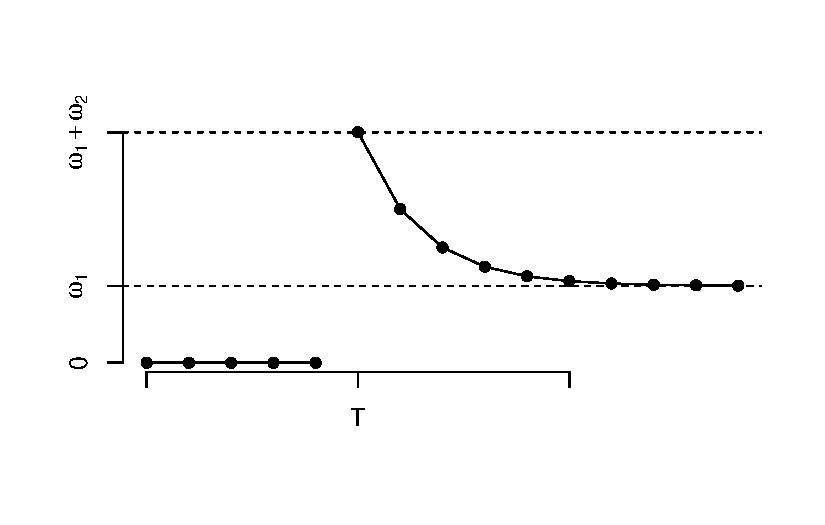
\includegraphics{intro_files/figure-pdf/unnamed-chunk-4-1.pdf}

}

\caption{1800 medidas da taxa cardíaca instantânea, em batidas por
minuto, de um indivíduo.}

}

\end{minipage}%

\end{figure}

\hypertarget{produto-interno-brupo-brasileiro}{%
\subsection{Produto Interno Brupo
Brasileiro}\label{produto-interno-brupo-brasileiro}}

\begin{Shaded}
\begin{Highlighting}[]
\FunctionTok{ts.plot}\NormalTok{(PIB)}
\end{Highlighting}
\end{Shaded}

\begin{figure}

\begin{minipage}[t]{\linewidth}

{\centering 

\raisebox{-\height}{

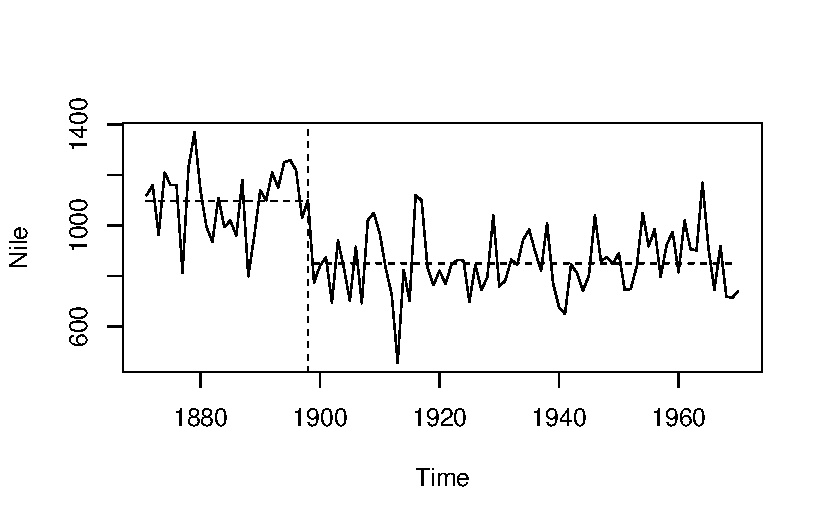
\includegraphics{intro_files/figure-pdf/unnamed-chunk-5-1.pdf}

}

\caption{PIB entre 1967 e 2014 corrigidos pelo valor do dólar em
4/2015.}

}

\end{minipage}%

\end{figure}

\hypertarget{mortes-por-doenuxe7as-pulmonares-no-reino-unido}{%
\subsection{Mortes por doenças pulmonares no Reino
Unido}\label{mortes-por-doenuxe7as-pulmonares-no-reino-unido}}

\begin{Shaded}
\begin{Highlighting}[]
\FunctionTok{ts.plot}\NormalTok{(ldeaths)}
\end{Highlighting}
\end{Shaded}

\begin{figure}

\begin{minipage}[t]{\linewidth}

{\centering 

\raisebox{-\height}{

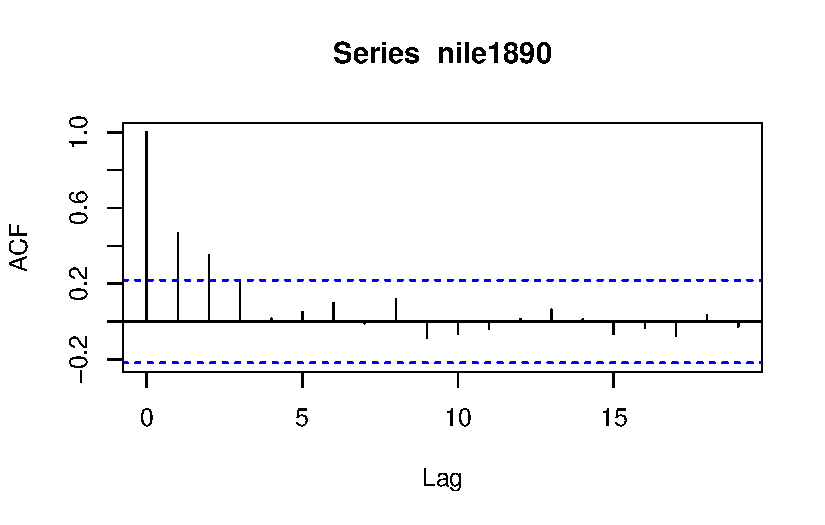
\includegraphics{intro_files/figure-pdf/unnamed-chunk-6-1.pdf}

}

\caption{PIB entre 1967 e 2014 corrigidos pelo valor do dólar em
4/2015.}

}

\end{minipage}%

\end{figure}

\bookmarksetup{startatroot}

\hypertarget{summary}{%
\chapter{Summary}\label{summary}}

In summary, this book has no content whatsoever.

\begin{Shaded}
\begin{Highlighting}[]
\DecValTok{1} \SpecialCharTok{+} \DecValTok{1}
\end{Highlighting}
\end{Shaded}

\begin{verbatim}
[1] 2
\end{verbatim}

\bookmarksetup{startatroot}

\hypertarget{suxe9ries-estacionuxe1rias}{%
\chapter{Séries Estacionárias}\label{suxe9ries-estacionuxe1rias}}

Uma coleção do tipo \(\{x(t),t\in\mathcal{T}\}\),
\(\mathcal{T}\subseteq \mathbb{R}\), onde \(x(t)\) é uma variável
aleatória para cada \(t\) fixado, é denominada processo estocástico.

Um processo estocástico é dito ser fortemente estacionário se sua
distribuição é invariante ao índice. Portanto, para qualquer
\(t_1,\ldots,t_k\), a distribuição de \(x(t_1),\ldots,x(t_k)\) é a mesma
de \(x(t_1+h),\ldots,x(t_k+h)\).

\begin{example}[]\protect\hypertarget{exm-serie_estacionaria_1}{}\label{exm-serie_estacionaria_1}

Se \(x(t)\sim \hbox{Normal}(0,1)\) e \(x(t)\) é independente de \(x(s)\)
para todo \(t\neq s\), então, para qualquer \(t_1,\ldots,t_k\),

\[\begin{align}P(x(t_1)<x_1,\ldots,x(t_k)<x_k)&=\prod_{i=1}^k P(x(t_i)<x_i)=\prod_{i=1}^k P(x(t_i+h)<x_i)\\&=P(x(t_1+h)<x_1,\ldots,x(t_k+h)<x_k)\end{align}\]
logo, \(\{x(t),t\in \mathbb{R}\}\) é um processo fortemente
estacionário. \(\blacksquare\)

\end{example}

\begin{theorem}[]\protect\hypertarget{thm-exm_estacionaria2}{}\label{thm-exm_estacionaria2}

Seja \(\{x(t),t\in\mathbb{N}\}\) um processo estocástico com
\[x(t)= x_{(t-1)}+\varepsilon_t,\;\;\varepsilon_t\sim\hbox{Normal}(0,1),\]
para \(t=1,2,\ldots\) com a condição de que
\(x_0\sim\hbox{Normal}(0,1)\) e que
\(Cov(\varepsilon_t,\varepsilon_s)=0\;\;\forall s\neq t\). Então,
\[x_t=x_{t-1}+\varepsilon_{t}=\cdots=x_0+\sum_{j=1}^t\varepsilon_t\sim\hbox{Normal}(0,t+1).\]
Como \(x_t\sim\hbox{Normal}(0,t+1)\) e, para qualquer \(h>0\),
\(x_{t+h}\sim\hbox{Normal}(0,t+h+1)\), temos que este processo não é
fortemente estacionário. \(\blacksquare\)

\end{theorem}

\begin{definition}[]\protect\hypertarget{def-fracamente}{}\label{def-fracamente}

Um processo estocástico \(\{y_t\}\) é dito ser fracamente estacionário
(ou de segunda ordem) se \[\begin{align*}
    E(y_t)&=\mu,\\
    Var(y_t)&=\nu,\\ 
    Cov(y_t,y_s)&=E(y_ty_s)-E(y_t)E(y_s)=\gamma(t-s)
    \end{align*}\] onde \(\mu\) e \(\nu\) são constantes independentes
de \(t\) e \(\gamma(t-s)\) depende de \(t\) e \(s\) somente através da
diferença \(|t-s|\). \(\blacksquare\)

\end{definition}

\begin{example}[]\protect\hypertarget{exm-fracamente1}{}\label{exm-fracamente1}

Considere o processo estocástico \(\{x(t),t\in\mathbb{N}\}\), onde
\[x(t) = \varepsilon(t) +\frac{1}{2}\varepsilon(t-1)
\] onde \(\varepsilon(t)\sim\hbox{Normal}(0,\nu)\) para \(t=1,\ldots\),
\(\varepsilon(t)\) é independente de \(\varepsilon(s)\) para todo
\(s\neq t\) e \(\varepsilon(0)=0\). Então: \[\begin{align}
E(x(t))&=E(\varepsilon(t))+\frac{1}{2}E(\varepsilon(t-1))=0\\
Var(x(t))&=Var(\varepsilon(t))+\frac{1}{4}Var(\varepsilon(t-1))=\frac{5}{4}\nu
\end{align}
\] e \[\begin{align}
          Cov(x(t),x(t+h))&=Cov\left(\varepsilon(t)+\frac{1}{2}\varepsilon(t-1),\varepsilon(t+h)+\frac{1}{2}\varepsilon(t+h-1)\right)\\
          &=Cov\left(\varepsilon(t),\varepsilon(t+h)\right)+\frac{1}{2}Cov\left(\varepsilon(t),\varepsilon(t+h-1)\right)\\
          &+\frac{1}{2}Cov\left(\varepsilon(t-1),\varepsilon(t+h)\right)+\frac{1}{4}Cov\left(\varepsilon(t-1),\varepsilon(t+h-1)\right)\\
          &=\left\{ \begin{array}{ll}
          \frac{4}{5}\nu,&\; h = 0 \\         
          \frac{1}{2}\nu,&\; |h|=1,\\
          0,&\;\hbox{caso contrário.}
          \end{array} \right.
    \end{align}\] Portanto, o processo é fracamente estacionáriao.
\(\blacksquare\)

\end{example}

Quando \(\mathcal{T}=\{t\in D\subseteq \mathbb{Z}\}\), utiliza-se a
notação \(x(t)=x_t\). Além disso, se \(t\) pode ser interpretado como
tempo, \(x_t\) é uma série temporal. Uma série temporal é dita ser
estacionária se ela é fracamente estacionária e o mesmo princípio se
aplica nessas notas de aula.

\hypertarget{ruuxeddo-branco}{%
\section{Ruído branco}\label{ruuxeddo-branco}}

\begin{definition}[]\protect\hypertarget{def-ruido_branco}{}\label{def-ruido_branco}

A Série \(x_t\) é dita ser um ruído branco se \[\begin{equation}
        Cov(x_t,x_s)=0,
        \end{equation}\] para todo \(t\neq s\). \(\blacksquare\)

\end{definition}

É imediato que o ruído branco é uma série temporal estacionária. Se
\(x_t\sim\hbox{Normal}(0,\sigma^2)\) é um ruído branco, então \(x_t\) é
independente de \(x_s\) para todo \(t\neq s\).

\bookmarksetup{startatroot}

\hypertarget{defasagens-e-autocorrelauxe7uxe3o}{%
\chapter{Defasagens e
autocorrelação}\label{defasagens-e-autocorrelauxe7uxe3o}}

\hypertarget{gruxe1fico-de-defasagens}{%
\section{Gráfico de Defasagens}\label{gruxe1fico-de-defasagens}}

Denomina-se por \textbf{defasagem} \(h\) (\emph{lag}, em inglês), um
atraso em \(h\) nos índices da série temporal. A tabela abaixo ilustra
algumas defasagens para a série \(x_1,\ldots,x_5\)

\begin{longtable}[]{@{}llll@{}}
\toprule\noalign{}
Série original & \(h=1\) & \(h=2\) & \(h=3\) \\
\midrule\noalign{}
\endhead
\bottomrule\noalign{}
\endlastfoot
\(x_1\) & & & \\
\(x_2\) & \(x_1\) & & \\
\(x_3\) & \(x_2\) & \(x_1\) & \\
\(x_4\) & \(x_3\) & \(x_2\) & \(x_1\) \\
\(x_5\) & \(x_4\) & \(x_3\) & \(x_2\) \\
\end{longtable}

Conforme dito anteriormente, a existência de uma estrutura de
dependência entre \(x_t\) e \(x_{t-h}\) permite que a série observada
seja utilizada para realizar previsões. Uma ferramenta exploratória
interessante para analisar esse tipo de estrutura é gráfico de
defasagens (no inglês \emph{lag plot}). Trata-se de um diagrama de
dispersão entre a série original e a série defasada, para algum \(h\)
fixado. Abaixo apresenta-se a série de embarques e desembraques no
aeroporo Eduardo Gomes para as 4 primeiras defasagens. Os números
representam a ordem (temporal) dos pares do diagrama e a linha cinza
pontilha é a reta \(y=x\).

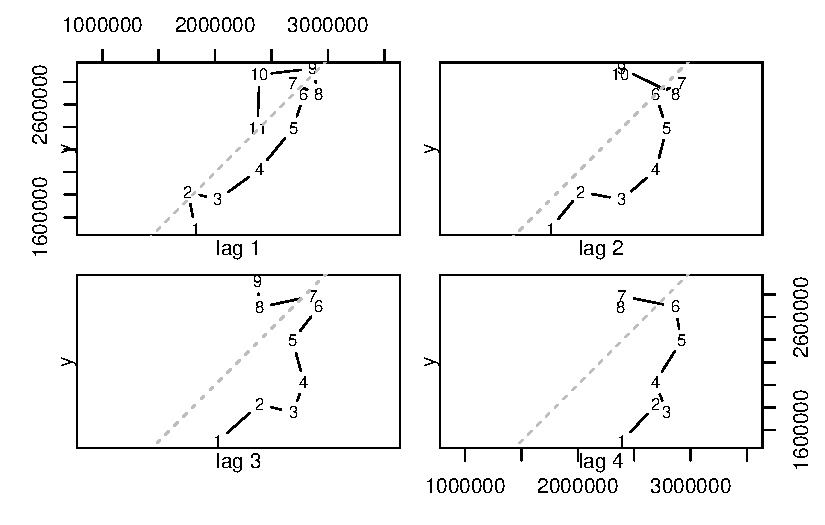
\includegraphics{acf_files/figure-pdf/unnamed-chunk-1-1.pdf}

Abaixo, a figura mostra o gráfico de defasagens para \(h=1,2,3,12\)
considerando a série de mortes por doenças pulmonares no Reino Unido.

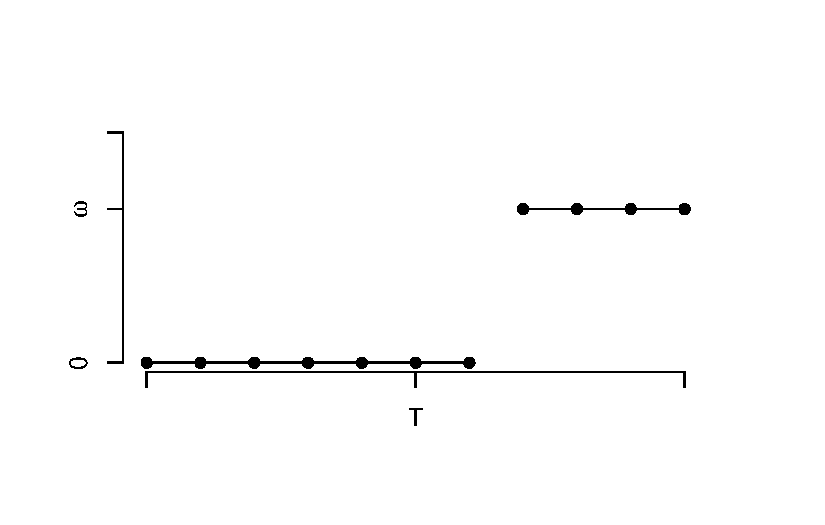
\includegraphics{acf_files/figure-pdf/unnamed-chunk-2-1.pdf}

\hypertarget{a-funuxe7uxe3o-de-autocorrelauxe7uxe3o}{%
\section{A função de
autocorrelação}\label{a-funuxe7uxe3o-de-autocorrelauxe7uxe3o}}

\begin{definition}[]\protect\hypertarget{def-autocovariancia}{}\label{def-autocovariancia}

A função de autocovariância da série temporal \(x_t\) é dada por
\[\begin{equation}
          \gamma(s,t) = Cov(x_t,x_s)=E\left[(x_t-\mu_t)(x_s-\mu_s)\right],
        \end{equation}\] para todo \(s,t\) com \(\mu_j=E(y_j)\) e sua
respectiva função de autocorrelção é dada por \[\begin{equation}
        \rho(s,t)=\frac{\gamma(s,t)}{\sqrt{\gamma(s,s)\gamma(t,t)}}
        \end{equation}\]

\end{definition}

\begin{example}[]\protect\hypertarget{exm-acf1}{}\label{exm-acf1}

Considere a série temporal
\[x_t= x_{t-1}+\varepsilon_t,\;\;\varepsilon_t\sim\hbox{Normal}(0,1),\]
para \(t=1,2,\ldots\) com a condição de que \(x_0=0\) e que
\(Cov(\varepsilon_t,\varepsilon_s)=0\;\;\forall s\neq t\). É imediato
que \[\begin{equation}
    x_{t}=\sum_{j=1}^{t}\varepsilon_{j},
    \end{equation}\] o que implica em \(x_t\sim\hbox{Normal}(0,t)\).
Portanto, \[\begin{align}
        E(x_t)&=0\\
        Var(x_t)&=t.
        \end{align}\] Além disso, \[\begin{align*}
    \gamma(t,t-h)&=Cov(x_t,x_{t-h})=Cov\left(\sum_{i=1}^{t}\varepsilon_{i},\sum_{j=1}^{t-h}\varepsilon_{j}\right)\\
    &=\sum_{i=1}^{t}\sum_{j=1}^{t-h}Cov\left(\varepsilon_{i},\varepsilon_{j}\right)=\sum_{i=1}^{t-h}Cov(\varepsilon_i,\varepsilon_i)\\
    &=t-h
    \end{align*}\] e \[\begin{equation}
    \rho(t,t-h)=\frac{\gamma(t,t-h)}{\sqrt{\gamma(t,t)\gamma(t-h,t-h)}}=\frac{t-h}{\sqrt{t(t-h)}}=\sqrt{1-\frac{h}{t}}
    \end{equation}\] A figura abaixo mostra o gráfico da função de
autocorrelação desse processo, considerando uma série de tamanho 100.
Note que a série é mais dependente dos valores atuais, embora ainda
possua uma autocorrelação alta para defasagens elevadas.

\begin{Shaded}
\begin{Highlighting}[]
\FunctionTok{curve}\NormalTok{( }\FunctionTok{sqrt}\NormalTok{(}\DecValTok{1}\SpecialCharTok{{-}}\NormalTok{x}\SpecialCharTok{/}\DecValTok{100}\NormalTok{),}\DecValTok{0}\NormalTok{,}\DecValTok{99}\NormalTok{, }\AttributeTok{xlab=} \StringTok{\textquotesingle{}Defasagem\textquotesingle{}}\NormalTok{, }\AttributeTok{ylab =} \StringTok{\textquotesingle{}Autocorrelação\textquotesingle{}}\NormalTok{)}
\end{Highlighting}
\end{Shaded}

\begin{figure}

\begin{minipage}[t]{\linewidth}

{\centering 

\raisebox{-\height}{

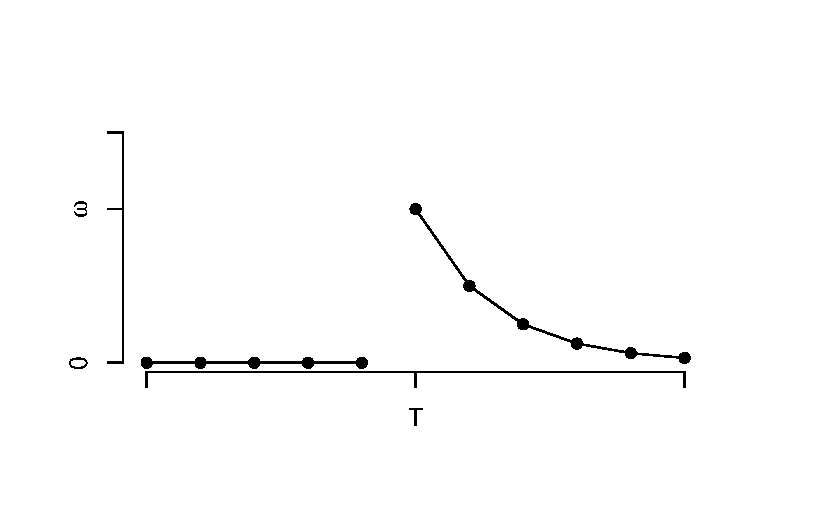
\includegraphics{acf_files/figure-pdf/unnamed-chunk-3-1.pdf}

}

\caption{Função de autocorrelação do Exemplo Example~\ref{exm-acf1},
para t=100}

}

\end{minipage}%

\end{figure}

\(\blacksquare\)

\end{example}

Para uma série estacionária, tem-se que \(E(x_t)=\mu\) para todo \(t\),
logo \[\begin{equation}
        \gamma(t-s) = Cov(y_t,y_s)=E\left[(y_t-\mu)(y_s-\mu)\right].
\end{equation}\] Fazendo \(h=t-s\), tem-se \[\begin{equation}
            \gamma(h)=Cov(y_t,y_{t-h}).
        \end{equation}\]

A função de autocorrelação (ACF) para um processo estacionário é
\[\begin{equation}
                \rho(h)=\frac{\gamma(h)}{\gamma(0)}
\end{equation}\] e ela mede a dependência linear entre \(y_t\) e os
valores defasados da série.Sempre será verdade que \(\rho\in[-1,1]\),
\(\rho(h)=\rho(-h)\) e, se \(y_{t+h}\) é independente de \(y_t\), então
\(\rho(h)=0\).

::: \{\#exm-acf2\} Considere novamente a série temporal \[\begin{align}
    x_t = \varepsilon_t +\frac{1}{2}\varepsilon_{t-1} \label{exer1}
    \end{align}\] onde \(\varepsilon_t\sim\hbox{Normal}(0,\nu)\) para
\(t=1,\ldots\), \(\varepsilon_t\) é independente de \(\varepsilon_s\)
para todo \(s\neq t\) e \(\varepsilon_0=0\). Já foi mostrado que
\[\begin{align}
    E(x_t)&=E(\varepsilon_t)+\frac{1}{2}E(\varepsilon_{t-1})=0\\
    Var(x_t)&=Var(\varepsilon_t)+\frac{1}{4}Var(\varepsilon_{t-1})=\frac{5}{4}\nu\\
    \gamma(h)&=\left\{ \begin{array}{ll}
    \frac{5}{4}\nu,&\; h = 0 \\       
    \frac{1}{2}\nu,&\; |h|=1,\\
    0,&\;\hbox{caso contrário.}
    \end{array} \right.
    \end{align}
\]\\
Portanto, \[\begin{align}
    \rho(h)&=\frac{\gamma(h)}{\gamma(0)}=\left\{ \begin{array}{ll}
    1,&\; h = 0 \\        
    \frac{2}{5},&\; |h|=1,\\
    0,&\;\hbox{caso contrário.}
    \end{array} \right.
    \end{align}\]

\bookmarksetup{startatroot}

\hypertarget{references}{%
\chapter*{References}\label{references}}
\addcontentsline{toc}{chapter}{References}

\markboth{References}{References}

\hypertarget{refs}{}
\begin{CSLReferences}{0}{0}
\end{CSLReferences}



\end{document}
